\section{Results}



Results of sin(x)

	\begin{figure}[h]
	\includegraphics[width=1.1\linewidth]{sin300_calc.pdf}
	\caption{Simplistic view of CPU and RAM.} \label{fig:1a}
	\end{figure}
	\begin{figure}
	\includegraphics[width=1.1\linewidth]{sin300_exact.pdf}
	\caption{More realistic view of CPU and RAM.} \label{fig:1b}
	\end{figure}
	\begin{figure}
	\centering
	\includegraphics[width=1.1\linewidth]{sin300_diff.pdf}
	\caption{More realistic view of CPU and RAM.} \label{fig:1b}
	\end{figure}


Result of dipole (compare to monopole)

	\begin{figure}[h]
	\centering
	\center
	\includegraphics[width=1.1\linewidth]{dipole_contours.pdf}
	\caption{Fitting a $1/r^2$ curve to the calculated dipole potential.} \label{fig:dipolefit}
	\end{figure}

	\begin{figure}[h]
	\centering
	\includegraphics[width=0.7\linewidth]{dipole_field.pdf}
	\caption{Fitting a $1/r^2$ curve to the calculated dipole potential.} \label{fig:dipolefit}
	\end{figure}


	\begin{figure}[h]
	\centering
	\includegraphics[width=\linewidth]{dipole_fit.pdf}
	\caption{Fitting a $1/r^2$ curve to the calculated dipole potential.} \label{fig:dipolefit}
	\end{figure}

	Performance Results

\begin{figure}
	\centering
	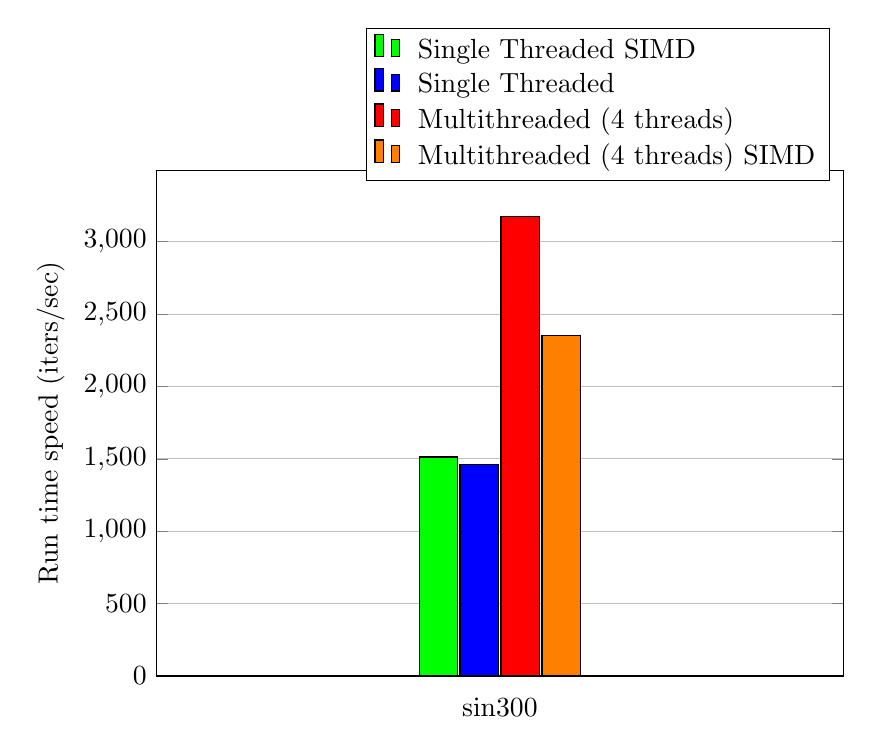
\begin{tikzpicture}
    \begin{axis}[
        symbolic x coords={sin300, sin1000},
        xtick=data,
        major x tick style = transparent,
        width  = 0.85*\textwidth,
        height = 8cm,
        major x tick style = transparent,
        ybar=2*\pgflinewidth,
        bar width=14pt,
        ymajorgrids = true,
        ylabel = {Run time speed (iters/sec)},
        xtick = data,
        scaled y ticks = false,
        enlarge x limits=0.25,
        ymin=0,
        legend cell align=left,
		legend style={
	        anchor=south east,
	        column sep=1ex
	    },
        ]
	\addplot[ybar,fill=green,mark=none] coordinates {(sin300,   1513.05)};
	\addplot[ybar,fill=blue,mark=none] coordinates {(sin300,   1459.24)};
	\addplot[ybar,fill=red] coordinates {(sin300,   3174.49)};
	\addplot[ybar,fill=orange] coordinates {(sin300,   2354.03)};
	\legend{Single Threaded SIMD, Single Threaded, Multithreaded (4 threads), Multithreaded (4 threads) SIMD}
\end{axis}
\end{tikzpicture}
\end{figure}
